\section{Characterization method and results}
\label{Method}
The setup of the experiment and preanalysis are discussed in sec.~\ref{sec:laserstage}. Analysis method and results of parameters are introduced in the following sections.
\subsection{Setup and preanalysis}
\label{sec:laserstage}

To yield single photoelectron (SPE) events, the laser intensity was adjusted to a level only about one out of 20 triggers lead to a signal. The window size $T_{\mathrm{wave}}$ is set to \SI{10400}{ns} and the rising edge of trigger waveform is at about \SI{200}{ns}, which reserves a time interval for pre-pulse analysis. The trigger from the laser system is a step wave, of which the vertical center of rising edge is linearly interpolated to get the trigger time $t_{\mathrm{trig}}$ as shown in Fig.~\ref{fig:triggertime}.
\begin{figure}[!htbp]
    \centering
    \includegraphics[width=\LF\textwidth]{figures/method/triggerwave.pdf}
    \caption{A waveform and the trigger signal in the experiment. The orange line is the trigger waveform. Two black horizontal dash lines are the upper and lower values of the step wave. The green cross point is the interpolation for trigger time. The blue solid line shows the PMT waveform with a signal and the blue dash line is the baseline. Red and green vertical dash lines are the time of 10\% of the rising edge and the pulse peak. The vertical green line indicates the peak position of the pulse candidate. The horizontal blue dash line and horizontal violet dash line are the baseline and amplitude threshold. The rise time and fall time are the width of the pink and green rectangle, of which start and end time are linearly interpolated as 10\% and 90\% of rising and falling edges.}
    \label{fig:triggertime}
\end{figure}

The preanalysis window is set as $t_{\mathrm{trig}}$ to $T_{\mathrm{wave}}=$\SI{600}{ns}. For \SI{20}{kHz} dark noise rate, the number of dark noise pulses in each waveform obeys Poisson distribution with expectation being about 0.008 while the number of laser pulse events is about 0.05, which dominate the dataset. The peak time $t_p$ is the position of minimum in each waveform as shown in Fig.~\ref{fig:triggertime}. Because the maximum pulse is selected in each waveform, the expected charge distribution is the distribution of $\max_n^N(C_n)$, in which $C_n$ is the charge of nth PE and $N$ is the number of pulses in a waveform. The charge bias caused by multi-pulse is omitted because of the small ratio of multi-pulse cases.

\begin{figure}[!htbp]
    \centering
    \includegraphics[width=\LF\textwidth,page=1]{figures/method/noisebaseline697_219908_2.pdf}
    \caption{A very large waveform example. The vertical green line indicates the peak position of the pulse candidate. The horizontal blue dash line and horizontal violet dash line are the baseline and amplitude threshold. The rise time and fall time are the width of the pink and green rectangle, of which start and end time are linearly interpolated as 10\% and 90\% of rising and falling edges.}
    \label{fig:baseline1}
\end{figure}

Due to the offset mentioned in sec.~\ref{sec:setup}, the value of the baseline is not zero. Potential signals are removed using a baseline threshold filter, as horizonal dash line shown in Fig.~\ref{fig:triggertime}, from an interval of the time window $[-t_s,-10\mathrm{ns}]$($t_s\leq200\mathrm{ns}$) and $[t_p+100\mathrm{ns},t_p+200\mathrm{ns}]$ relative to pulse peak $t_p$. The selected areas are cut off \SI{10}{ns} at both ends to remove the rising edge and falling edge of potential pulses. The baseline $\mu_b$ and fluctuation $\sigma_b$ are estimated as average and the standard deviation of the rest waveform. A gaussian function G$(\mu_{t0},\sigma_{t0})$ is unbinned fitted to the distribution of $t_p-t_{\mathrm{trig}}$ of pulses whose peak is larger than \SI{5}{ADC} for each PMT. To reduces the impact of dark noise, a shorter window $[\mu_{t0}-5\sigma_{t0}, \mu_{t0}+5\sigma_{t0}]$ is used to calculate all the characterizations include $t_p$.

\subsection{Peak and charge spectrum}
\label{sec:noisepeak}

The peak $V_p$ of a pulse is the difference between the baseline and minimum of the pulse. Considering the rise time and fall time distribution, the charge of a pulse is calculated using integration in a time window $[-15, 75]$\,ns relative to the peak location $t_p$ of the signal as illustrated in the pink region in Fig.~\ref{fig:triggertime}, with integration window $T_s$ is \SI{90}{ns}. The equivalent charge $C_{\mathrm{equ}}$ is defined as the summation of the amplitudes without baseline in the integration interval. Due to the input impedance being \SI{50}{\Omega} \cite{CAENV1751}, the true charge $C$ of the pulse is $\frac{C_{\mathrm{equ}}}{50 \Omega}$.

Fig.~\ref{fig:triggercharge} shows the distribution of the equivalent charge of an MCP-PMT. The pedestal is a set of waveforms with no signal, of which the equivalent charge is the summation of baseline and obeys Gaussian distribution $G(0, T_s\sigma_b^2)$, in which $\sigma_b$ is the standard deviation of the white noise of baseline mentioned in sec.\ref{sec:laserstage}. The charge of the main peak in charge distribution $C_1$ is fitted in sec.\ref{sec:noisegain}. To remove the influence of the pedestal, pulses of which peaks are larger than \SI{3}{ADC} and charge are larger than 0.25$C_1$ are selected. The charge of selected pulses is noted as $C_{\mathrm{sel}}$. Mean $\mu_{C}=\mathrm{E}(C_{\mathrm{sel}})$ and sample variance $s^2_{C}=\mathrm{Var}[C_{\mathrm{sel}}]$ of $C_{\mathrm{sel}}$ are calculated to represent the characteristics of the total charge distribution of MCP-PMTs. Due to the influence of long tail, the $\mu_{C}$ is larger than $C_1$. The physical model and solution of the long tail in charge distribution will be discussed in future work.

The peak amplitude distribution with \SI{1}{ADC} bin width is illustrated in Fig.~\ref{fig:triggerpeak}, which shows \SI{3}{ADC} and 0.25$C_1$ threshold are complementary to exclude some noise with small peak height but large charge.

\begin{figure}[!htbp]
    \centering
    \begin{subfigure}[b]{\SF\textwidth}
        \includegraphics[width=\textwidth]{figures/method/triggercharge.pdf}
        \caption{}%PM
        \label{fig:triggercharge}
    \end{subfigure}
    \begin{subfigure}[b]{\SF\textwidth}
        \includegraphics[width=\textwidth]{figures/method/triggerpeak.pdf}
        \caption{}%PM
        \label{fig:triggerpeak}
    \end{subfigure}
    \caption{(a) Charge distribution of an example MCP-PMT in the laser stage. (b) Peak distribution of an example MCP-PMT in the laser stage. The vertical green dash line is the threshold cut for the peak. The orange histogram is the selected entries with charge selection.}
\end{figure}

\subsection{Gain and single PE resolution}
\label{sec:noisegain}

There exists a long tail in charge distribution as shown in the histogram in Fig.~\ref{fig:triggercharge}. To describe the energy resolution of the main peak of the charge distribution, a gaussian function G$(C_1,\sigma^2_{C})$ is used to fit the binned data in an interval $[0.65C_1, 1.35C_1]$ via the modified least-square (MLS) method \cite{Cowan1998StatisticalDA} to capture the main peak of charge distribution of the single PE as shown in Fig.~\ref{fig:triggercharge}. The gain of main peak and gain of total charge of single PE are calculated as $G_1=\frac{C_1}{e\times 50\Omega}$ and $G= \frac{\mu_{C_t}}{e\times 50\Omega}$,in which $e$ is the charge of an electron. The main peak resolution and the total charge resolution are defined as $\mathrm{Res}_1=\frac{\sigma_{C}}{C_1}$ and $\mathrm{Res}=\frac{\sqrt{s^2_{C}}}{\mu_{C}}$.

Fig.~\ref{fig:totalchargeCompare} shows the 2d distribution of gain and resolution. $G$ is about 2 times $G_1$ for MCP-PMT, which should be considered in waveform analysis. Although $\mathrm{Res}_1$ of MCP-PMT is about 0.25, the long tail leads that $\mathrm{Res}$ is about 0.69, worse than the reference PMT.

\begin{figure}[!htbp]
    \centering
    \includegraphics[width=\MF\textwidth]{figures/result/gainres.pdf}
    \caption{Gain and resolution of total charge and main peak in the laser stage. Geen points represent reference PMT and red points represent MCP-PMTs. Cross markers represent $G_1$ and $\mathrm{Res}_1$. Plus markers represent $G$ and $\mathrm{Res}$.}
    \label{fig:totalchargeCompare}
\end{figure}

\subsection{Peak-to-valley (P/V) ratio}
A parabolic function is fitted to the valley based on the MLS method in the interval $[-0.15C_1, 0.25C_1]$ relative to the least count bin of histogram between pedestal and SPE peak as shown in Fig.~\ref{fig:triggercharge}. The local minimum $N_v$ of the charge spectrum is calculated as the minima of the parabolic function. The $N_p$ is the peak of the Gaussian function described in sec.~\ref{sec:noisegain}. The P/V ratio is equal to $\mathrm{P/V}=\frac{N_p}{N_v}$, which shows the ability to discriminate between electronic noise and true signal. The mean P/V ratio of MCP-PMT is about $5.79$ in the laser stage.

\subsection{Rise time, fall time, and full width at half maximum (FWHM)}
As shown in Fig.~\ref{fig:triggertime}, $t^{10}_r$, $t^{50}_r$, $t^{90}_r$ are the time of 10\%, 50\%, and 90\% $V_p$ in the rising edge and $t^{10}_f$, $t^{50}_f$, $t^{90}_f$ are the time of 10\%, 50\%, and 90\% $V_p$ in the falling edge which are acquired via linear interpolation method. The rise time, fall time, and FWHM are calculated as follows: $t_r = t^{90}_r - t^{10}_r$, $t_f = t^{10}_f - t^{90}_f$, $\mathrm{FWHM} = t^{50}_f - t^{50}_r$.

% \begin{figure}[!htbp]
%     \centering
%     \includegraphics[width=0.4\textwidth]{figures/method/triggerFWHM.pdf}
%     \caption{An example of time characteristics in the laser stage.}
%     \label{fig:triggerFWHM}
% \end{figure}

 Estimated rise time, fall time, and FWHM are $3.71\pm0.15$\,ns, $15.6\pm1.8$\,ns, and $9.07\pm0.63$\,ns for 9 MCP-PMT in the laser stage.

\subsection{Transit time spread (TTS)}
The photoelectrons generated from cathode drift to the MCP in the electric field as shown in Fig.~\ref{fig:mcpelectron}. The drift time is determined by the initial kinetic of photoelectros and the electric field. A simple model consisting of a cathode, a focus dynode, and a MCP with \SI{0}{V}, \SI{480}{V}, and \SI{528}{V} is constructed to simulate the electric field and the electron trajectory. The drift times of the electrons at the top of PMT with \SI{0}{eV} and \SI{3}{eV} are about \SI{21}{ns} and \SI{18}{ns}. The electrons hitting in the channels of MCP are multiplied and generate observable signals, while the electrons hitting on the surface of MCP generate the secondary electrons (incluing elastic scattering electron), which drift in the electric field until rehitting on the MCP \cite{KM3NetTesting}. The transit time (TT) of a PE is composed of drift time and multiplication time.

\begin{figure}[!htbp]
    \centering
    \begin{subfigure}[t]{\SF\textwidth}
        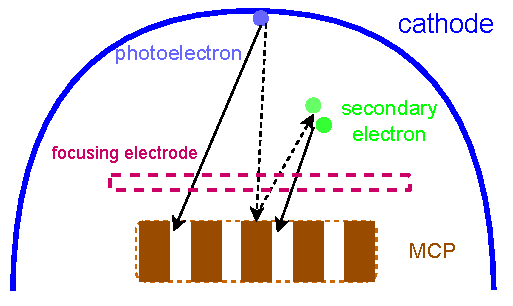
\includegraphics[width=\textwidth]{figures/method/MCPelectron.pdf}
        \caption{}%PM
        \label{fig:mcpelectron}
    \end{subfigure}
    \begin{subfigure}[t]{\SF\textwidth}
        \includegraphics[width=\textwidth]{figures/method/triggerTTS.pdf}
        \caption{}%PM
        \label{fig:triggerTTSLog}
    \end{subfigure}
    \caption{(a) The drift of electrons between cathode and MCP. (b) The distribution of TT with y-axis in logarithm sacle.}
\end{figure}

The TTS is the spread of TT, which represents the resolution of timing. The transit time cannot be measured directly, while the trigger time of the laser and time of pulse can be measured. A relative transit time $\mathrm{TT}_r$ is defined as the time difference between trigger time $t_{\mathrm{trig}}$ and $t_r^{10}$. The distribution of $\mathrm{TT}_r$ contain two slow falling edge in both side of the peak as shown in Fig.~\ref{fig:triggerTTSLog}. The tail before peak of TT distribution is due to large kinetic of photoelectron, which leads to larger charge response as shown in Fig.~\ref{fig:triggerTTS2d}. The tail in the other side is consisted of secondary electrons with a longer drift time, which may contain two pulses due to different drift time of secondary electrons as shown in Fig.~\ref{fig:triggerTT2pulse}. To describe the delayed pulse after main peak, the interval $[20\mathrm{ns},80\mathrm{ns}]$ related to $t_p$ is used to find pulses and the distribution in Fig.~\ref{fig:triggerTTlatepulse} illustrates the elastic scattering electrons gather at about \SI{40}{ns} after main pulse.

\begin{figure}[!htbp]
    \centering
    \begin{subfigure}[t]{\SF\textwidth}
        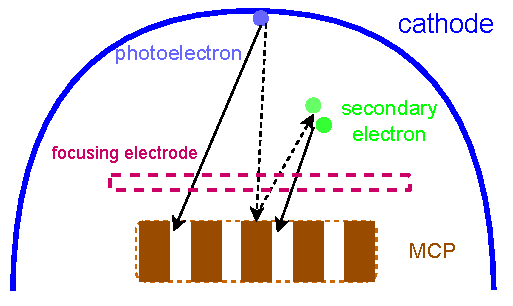
\includegraphics[width=\textwidth]{figures/method/MCPelectron.pdf}
        \caption{}%PM
        \label{fig:triggerTT2pulse}
    \end{subfigure}
    \begin{subfigure}[t]{\SF\textwidth}
        \includegraphics[width=\textwidth]{figures/method/triggerTTS.pdf}
        \caption{}%PM
        \label{fig:triggerTTlatepulse}
    \end{subfigure}
    \caption{(a) Double pulses example. (b) The delayed pulse distribution.}
\end{figure}

Main pulse and tail before main pulse are modeled with Gaussian function $N_tG(\mu_{\mathrm{TT}},\sigma_{\mathrm{TT}}^2)$ and $N_LG(\mu_L,\sigma_L^2)$.Considering the distribution of kinetic energy of secondary electrons \cite{Furman,SecondElectron} and observered data, a phenomenological unphysical function $b_S+N_Se^{-\frac{t}{\tau_S}}$ is used to model the delayed pulse. Besides, to avoid the influence of unphysical function on $G(\mu_{\mathrm{TT}},\sigma_{\mathrm{TT}}^2)$, the function is translated to $\mu_{\mathrm{TT}}+2\sigma_{\mathrm{TT}}$.  As shown in Fig.~\ref{fig:triggerTTSLog} and Fig.~\ref{fig:triggerTTS}, the histogram of $\mathrm{TT}_r$ with \SI{0.5}{ns} bin width is binned fitted using following equation
\begin{equation}
    N_tG(\mu_{\mathrm{TT}},\sigma_{\mathrm{TT}}^2)+N_LG(\mu_L,\sigma_L^2)+H(\mu_{\mathrm{TT}}+2\sigma_{\mathrm{TT}})\left(b_S+N_Se^{-\frac{t-(\mu_{\mathrm{TT}}+2\sigma_{\mathrm{TT}})}{\tau_S}}\right)
\end{equation}
in which $H$ is heaviside function to limit the unphysical exponential function.TTS is defined as FWHM $2\sqrt{2\ln(2)}\sigma_{\mathrm{TT}}$ \cite{HAMAMATSUManual}. 

\begin{figure}[!htbp]
    \centering
    \begin{subfigure}[t]{\SF\textwidth}
        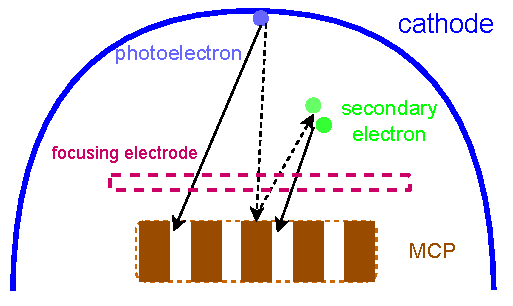
\includegraphics[width=\textwidth]{figures/method/MCPelectron.pdf}
        \caption{}%PM
        \label{fig:triggerTTS}
    \end{subfigure}
    \begin{subfigure}[t]{\SF\textwidth}
        \includegraphics[width=\textwidth]{figures/method/triggerTTS.pdf}
        \caption{}%PM
        \label{fig:triggerTTS2d}
    \end{subfigure}
    \caption{(a) The distribution of TT with y-axis in linear sacle. (b) The 2d distribution of TT and equivalent charge.}
\end{figure}

\subsection{Single electron response (SER)}
\begin{figure}
    \centering
    \includegraphics[width=\MF\textwidth]{figures/method/triggerSER.pdf}
    \caption{A fitting result of a pulse.}
    \label{fig:triggerser}
\end{figure}
To get a smooth single electron response (SER), the pulses are selected by dedicated cuts:
\begin{itemize}
    \item[1] The amplitude and charge of pulses should fulfill the criteria in sec.~\ref{sec:noisepeak}.
    \item[2] The FWHM of candidate pulses should exceed \SI{5}{ns} to avoid noise.
    \item[3] To focus on the pulse in the main peak of charge distribution and remove the influence of fluctuation, a charge filter $[0.5C_1, 1000\mathrm{ADC\cdot ns}]$ is used for reliable results.
\end{itemize}

A gaussian function convoluted with an exponential function Equ~\eqref{equ:ser} is used to fit the SER which is shown in Fig.~\ref{fig:triggerser}.

\begin{equation}
    \label{equ:ser}
    \mathrm{Gaus}(0,\sigma_{\mathrm{ser}}^2)\otimes\theta(t-\mu_{\mathrm{ser}})\frac{1}{\tau_{\mathrm{ser}}}e^{-\frac{t-\mu_{\mathrm{ser}}}{\tau_{\mathrm{ser}}}}
\end{equation}
in which $\theta(t)$ is the unit step function, $\mu_{\mathrm{ser}}$ is the time offset of pulse, $\sigma_{\mathrm{ser}}$ and $\tau_{\mathrm{ser}}$ model the shape feature of SER. The results of $\tau_{\mathrm{ser}}$ and $\sigma_{\mathrm{ser}}$ of 9 MCP-PMTs are shown in Fig.~\ref{fig:sigmaCompare}.
\begin{figure}[!htbp]
    \centering
    \includegraphics[width=\MF\textwidth]{figures/result/tausigma.pdf}
    \caption{$\tau$ versus $\sigma$ of 9 MCP-PMTs in the laser stage.}
    \label{fig:sigmaCompare}
\end{figure}


\subsection{Pre-pulse and after-pulse}

\begin{figure}
    \centering
    \includegraphics[width=\LF\textwidth]{figures/method/triggerAfterpulseSchema.pdf}
    \caption{Schema for searching after-pulses. Green and red vertical dash lines are the rising edge of trigger waveform and 10\% of rising edge of main pulse. The dark region is the interval for searching after-pulse.}
    \label{fig:afterpulseSchema}
\end{figure}

The generation of pre-pulses is due to photons hitting on the MCP or the first dynode directly rather than the photocathode \cite{JUNOMassTesting}. The amplitudes of pre-pulses are smaller than that of normal signals and pre-pulses appear before the main pulse about tens of nanoseconds \cite{JUNOMassTesting}. After-pulse is generated due to the ionization of gaseous impurities between the cathode and first dynode or MCP when photoelectrons go through \cite{Coates_1973}. These ions hit back on the photocathode and generate electrons. \ce{H^+}, \ce{He^+}, \ce{O^+} are the major ions contributing to after-pulse and the relation between time and ions (\ce{^Z_MX}) is $\sqrt{\frac{M}{Z}}$, in which $M$ and $Z$ are the mass and charge of ions \cite{Coates_1973}. Due to these ions being heavier than the electron, the travel time is in the scale of \si{us}\footnote{The velocity of ions is about \SI{1000}{km/s} and size of PMT is about \SI{0.1}{m}, thus the transit time is in the scale of about \SI{0.1}{us}.}. The after-pulse is searched in a window \SIrange{100}{10000}{ns} after the main pulse as shown in Fig.~\ref{fig:afterpulseSchema}. The $t$ and $Q$ are calculated as the max peak and integrated in the $[-15,75]$ ns window relative to the peak position as shown violet area in Fig.~\ref{fig:afterpulseSchema}.

\begin{figure}[!htbp]
    \centering
    \includegraphics[width=\LF\textwidth]{figures/method/triggerAfterpulse1d.pdf}
    \caption{Time distribution of pre-pulse and after-pulse. The orange and blue histograms are pre-pulse and after-pulse. The green line is the fit result for the distribution of after-pulse. The blank area around the \SI{0}{ns} is the main pulse which is not shown in this figure.}
    \label{fig:afterpulse1d}
\end{figure}
% waveform analysis

After-pulse is categorized into several kinds. Fig.~\ref{fig:afterpulse1d} indicates 4 typical after-pulse peaks in time around \SI{300}{ns}, \SI{500}{ns}, \SI{1200}{ns} and \SI{1700}{ns}, of which ratio is about $1:\sqrt{3}:\sqrt{16}:\sqrt{32}$. Besides, the peak at about \SI{100}{ns} is influenced by the main pulse. Considering the different mass of ions, these peaks may originate from \ce{H^+}, \ce{He^{+}} or other unknown ions, \ce{O^+}, and \ce{O_2^+} or other unknown ions. Other similar works done by JUNO and KM3Net claimed the first peak is \ce{H_2^{+}} for the \SI{20}{inch} PMT \cite{Zhao:2022gks,KM3NetTesting}. Double Chooz proposed some assumptions including $H$ \cite{Haser_2013}. More work needs to be done for an advanced model.

The time distribution and ratio of different peaks in after-pulse distribution are parameterized using 4 gaussian functions to model the four peaks as shown in Fig.~\ref{fig:afterpulse1d} and the fit equation is as follows

\begin{equation}
    \label{equ:afterpulse}
    N_{\mathrm{trig}}\sum_{i=1}^{4}{A_iG(t_i,\sigma_i^2)}
\end{equation}
in which $A_i$, $t_i$, and $\sigma_i$ are the ratio, time, and width of each peak of after-pulse. The fit results are shown in Fig.~\ref{fig:afterpulsePeak} and the ratios of 4 peaks vary greatly for different MCP-PMTs. Besides, there exist some areas that cannot be well modeled with Equ.\eqref{equ:afterpulse}, for example, the pedestal between the first and second peaks of after-pulse distribution. The mean and standard deviation of fit results are summarized in Table.~\ref{tab:afterpulse}. Due to the influence of after-pulses around the second peak, the standard deviation of $\sigma_2$ is very large.
\begin{figure}[!htbp]
    \centering
    \includegraphics[width=\MF\textwidth]{figures/result/afterpulse.pdf}
    \caption{Time and relative ratio of peaks of after-pulse ratios of 9 MCP-PMTs. 4 peak ratios are plotted along the time for each PMT.}
    \label{fig:afterpulsePeak}
\end{figure}
% \begin{figure}[!htbp]
%     \centering
%     \includegraphics[width=0.5\textwidth]{figures/method/triggerAfterpulse2d.pdf}
%     \caption{time and charge distribution of after pulse}
%     \label{fig:afterpulse2d}
% \end{figure}
% Fig.\ref{fig:afterpulse2d} indicates that the after pulse contains some very large signal in the specific peaks, which is different from the distribution of single PE.
\begin{table}
    \centering
    \caption{Parameters of after-pulse of 9 MCP-PMTs}
    \label{tab:afterpulse}
    \begin{tabular}{c|c|c|c|c}
        \hline
        &1st peak&2nd peak&3rd peak&4th peak\\
        $t_i$/ns&307$\pm$7&535$\pm$40&1194$\pm$34&1724$\pm$27\\
        $A_i/A_1$&1&0.53$\pm$0.22&0.96$\pm$0.44&1.9$\pm$1.2\\
        $\sigma_i$/ns&11$\pm$4&66$\pm$40&50$\pm$30&69$\pm$28\\
        \hline
    \end{tabular}
\end{table}

The ratio of pre-pulse $R_{\mathrm{pre}}$ is calculated in time interval [-200,-5]\,ns and after-pulse $R_{\mathrm{after}}$ is calculated in time interval [200,9800]\,ns as following equations

\begin{align}
    R_{\mathrm{pre}} = \frac{N_{\mathrm{pre}}}{N_t} - \mathrm{DCR}\cdot T_{\mathrm{pre}}\times10^{-6}\\
    R_{\mathrm{after}} = \frac{N_{\mathrm{after}}}{N_t} - \mathrm{DCR}\cdot T_{\mathrm{after}}\times10^{-6}
\end{align}
in which $T_{\mathrm{pre}}=200$\,ns, $T_{\mathrm{after}}=9600$\,ns, $N_{\mathrm{pre}}$ and $N_{\mathrm{after}}$ are the number of pre-pulses and after-pulses. Due to the ratio of pre-pulse is too small, some measured values are smaller than zero after deducting DCR as shown in Fig.~\ref{fig:prepulseCompare}.

\begin{figure}[!htbp]
    \centering
    \includegraphics[width=\MF\textwidth]{figures/result/preafterpulse.pdf}
    \caption{pre-pulse ratio versus after-pulse ratio.}
    \label{fig:prepulseCompare}
\end{figure}
\subsection{Dark count rate (DCR)}
The dark mainly noise comes from the spontaneous thermionic electron emitted from the photocathode \cite{KM3NetTesting}, which generates a pulse signal similar to a photoelectron. To discriminate the dark noise with fluctuation of baseline, pulses reach criteria in sec.\ref{sec:noisepeak} are considered as dark noise. The DCR equals the following equation

\begin{equation}
    \mathrm{DCR/kHz} = \frac{N_{\mathrm{noise}}}{N_{t}}\frac{1}{T_{\mathrm{wave}}/\mathrm{ns}}\times 10^{6}
\end{equation}
in which $N_{\mathrm{noise}}$ is the noise number and $N_{t}$ is the total number of waveforms. The DCRs of MCP-PMTs are illustrated in Fig.~\ref{fig:DCRCompare}.

\begin{figure}[!htbp]
    \centering
    \includegraphics[width=\MF\textwidth]{figures/result/DCRPDE.pdf}
    \caption{Relative PDE versus DCR of 9 MCP-PMTs.}
    \label{fig:DCRCompare}
\end{figure}

\subsection{Relative photon detection efficiency (PDE)}
The DCR is omitted in the PDE calculation due to the small ratio of dark noise. To measure PDE, the intensity of light and light allocation ratio of each channel of the laser splitter need to be calibrated. For example, JUNO fixed one reference PMT to calibrate the light intensity and other reference PMTs are circulated through all channels to calibrate the light allocation ratio \cite{Wonsak_2021}. A new method is designed to reduce the number of reference PMT to 1 PMT and combine all test runs to do the calibration in this work.

Note $n,j,k$ ($n=0,...,N-1, j=0,...,J-1, k=0,...,K-1$) is the indicator of the test run, channel of splitter and PMT. The intensity of light is $I_n$, light allocation ratio is $\alpha_j$ and PDE is $\eta_k$. Assume $\alpha_j$s are stable among different test runs. $N_t$ is the total number of waveforms. The photon numbers in each waveform obey Poisson distribution $\pi(p_{njk})$, in which $p_{njk}=I_n\alpha_j\eta_k$. The trigger rate of nth run, kth PMT in jth channel is

\begin{equation}
    \label{equ:pderate}
    R_{njk}=1-e^{-p_{njk}}
\end{equation}
For convenience, 0th PMT is the only one reference PMT. Note $\alpha_j^0=\frac{\alpha_j}{\alpha_0}$, $\eta_k^0=\frac{\eta_k}{\eta_0}$, $I_n^0=I_n\alpha_0\eta_0$, $i\equiv njk$. $p_{njk}$ can be transfer to Equ~\eqref{equ:pdelograte}

\begin{equation}
    \label{equ:pdelograte}
    \mathrm{log}(p_{i})=\mathrm{log}(I_0\alpha_0\eta_0)+\mathrm{log}(I_n^0)+\mathrm{log}(\alpha_j^0)+\mathrm{log}(\eta_k^0)
\end{equation}
The relationship between $R_{i}$ and parameters is

\begin{equation}
    \label{equ:linkfunction}
    R_{i}=1-e^{-e^{\mathrm{log}(I_0\alpha_0\eta_0)+\mathrm{log}(I_n^0)+\mathrm{log}(\alpha_j^0)+\mathrm{log}(\eta_k^0)}}
\end{equation}
The trigger number $N_{\mathrm{trig}}$ of kth PMT in nth run with jth splitter obey Binomial distribution $B(R_{i},N_{t_{i}})$, in which $N_{t_{i}}$ is total number of waveforms. To fit the parameters, a likelihood is constructed as follows

\begin{equation}
    \label{equ:likelihood}
    \mathcal{L}=\prod_{i}{R_{i}^{N_{\mathrm{trig}_{i}}}(1-R_{i})^{N_{t_{i}}-N_{\mathrm{trig}_{i}}}}
\end{equation}

The relationship in Equ.~\eqref{equ:linkfunction} matches the general linear model (GLM) of Binomial exponential family distribution with Cloglog link function\cite{glm}. The GLM is used to maximize the likelihood in Equ.~\eqref{equ:likelihood} and calculate the best value of $\mathrm{log}(\eta_k^0)$ and $\mathrm{log}(\alpha_k^0)$, which is used to calibrate relative photon detection efficiencies and splitter ratios. The results of PDE are shown in Fig.~\ref{fig:DCRCompare}. The mean of relative PDE is about $1.71$, which is obviously higher than the reference PMT.

The mean and standard deviation of parameters of 9 MCP-PMTs are summarized in Table~\ref{tab:summary}.
\begin{table}
    \centering
    \caption{charge and time characteristic of 9 MCP-PMTs}
    \label{tab:summary}
    \begin{tabular}{c| r @{$\pm$} l}
        Parameter&\multicolumn{2}{c}{$\mu\pm\sigma$}\\
        \hline
        $G_1$/1E7&1.19&0.07\\
        $G$/1E7&2.1&0.2\\
        $\mathrm{Res}_1$&0.25&0.02\\
        Res&0.69&0.03\\
        TTS/ns&1.82&0.09\\
        DCR/kHz&4.5&1.3\\
        $\tau_{\mathrm{ser}}$/ns&7.2&1.0\\
        $\sigma_{\mathrm{ser}}$/ns&1.62&0.06\\
        relative PDE&1.71&0.06\\
        $R_{\mathrm{pre}}$&0.0001&0.0002\\
        $R_{\mathrm{after}}$&0.02&0.01\\
        \hline
    \end{tabular}
\end{table}
